\chapter{Design}

%% Obviously you need to delete these lines when you have written up your text
% \begin{itemize}
% \item{} How you designed your solution
% \item{} Rationale for decisions
% \item{} Compare and contrast design with other approaches (related work) 
% \end{itemize}

%% Original from proposal
% The original technique and the proposed extensions will be implemented as two applications. The 
% first application will be used to generate the voxel-meshes that are needed by both techniques. The
% second application will perform the physics simulation. This approach was chosen to remove the need
% for voxelization, which can be a costly operation when implemented in a naive fashion, to occur at
% simulation run time.
%% End original

In order to support both the technique described by Muller \etal and the bezier extension, a data 
set of voxelized meshes will be required. WHile there are methods to compute the voxelization of a 
given mesh quite efficeiently, through the use of compute shaders or a method which takes advantage 
of oct-tree like solutions (TODO: find papers), These would be fairly time consuming to design, 
implement, and debug. Furthermore, both methods require a rigid-body physics simulation. Which will 
be the main focus for evaluating the efficiency and visual quality of both methods. As such, a 
naive approach will be takin for the voxelization process. An unfortunate draw back of this approach
will be the increased time it takes to voxelize a given mesh. To overcome this, the voxelization
will occur in a seperate application than the physics simulation and the voxelized meshes will be 
stored in a serialized format on disc for the physics simulation application to reference.

These two applications will have a significant amount of overlap in terms of functionality required.
Such as rendering, management of the various meshes and voxelmeshes, serialization, and various 
utilities. Due to this fact, a small library of common classes, interfaces, and utilities will be 
designed and implemented.

\section{Shared Library Design} \label{SharedLibrary}

%% old
% Due to the fact that a significant amount of functionality is shared between the Voxelization
% application and the Physics Simulation application, a shared library will be used. This shared
% library will contain the necessary implementations and interfaces needed by the two applications. 
% The contents of this library in relation to its use by the applications can be seen in figure
% \ref{fig:SharedLibraryUML}.
%% end old

% TODO: need to flesh this out a bit
The main components of the library are the MeshManager class, the serilization and 
de-serialization routines, the representation of meshes, voxel-meshes, and Bezier curves, and the
renderer.

%% TODO: maybe for future use
% \begin{figure}[h]
%   \centering
%   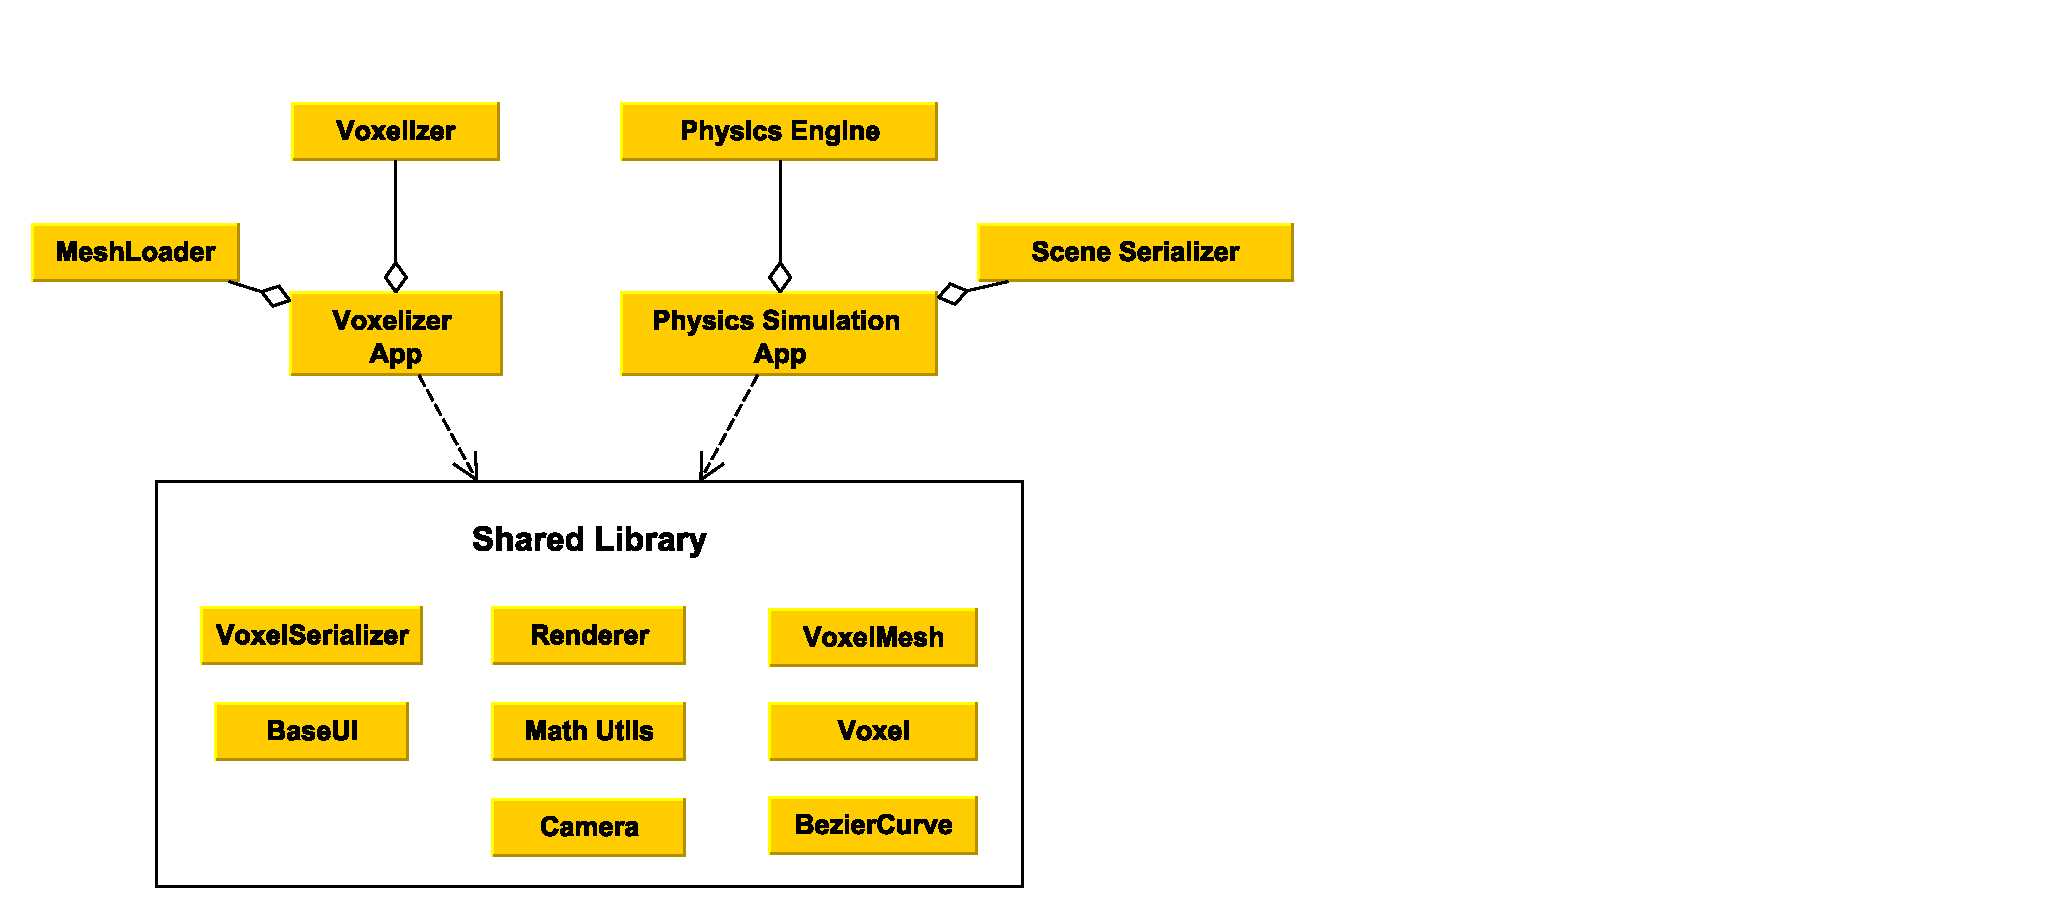
\includegraphics[width=0.8\textwidth, trim={0cm 0cm 15cm 0cm}]{SharedLibraryUML}
%   \caption{Shared Library UML Diagram}
%   \label{fig:SharedLibraryUML}
% \end{figure}

\subsubsection{MeshManager}
The MeshManager acts as a simple database for storing meshes and voxelmeshes. A UML describing its
basic structure can be seen in \ref{fig:MeshManagerUML}. When a Mesh is given to the MeshManager, a
MeshHandle will be returned to the callee. WHich will allow the Mesh to referenced in the future.
THis handle will also be used to submit VoxelMeshes, as both applications will require that Meshes 
are paired with their VoxelMesh representation. Both Meshes and VoxelMeshes will be stored in 
HashMaps with their respective handle as the key. The next available handle will also be tracked
to prevent duplicate handles from being used.

\begin{figure}[h]
  \centering
  \includegraphics[width=5cm]{example-image-a}
  % \includegraphics[height=5cm]{example-image-a}
  \caption{MeshManager UML Diagram}
  \label{fig:MeshManagerUML}
\end{figure}

\subsubsection{Serialization and De-Serialization}

The serialization interface will provide a way to convert meshes and voxel-meshes into a format 
which can then be read back from disk. This will provide the means for the voxelization application
to provide the data sets needed by the physics application. Rather than inventing a new file format 
for serialization, an existing format will be used. Ideally, this format will be human readable with 
plenty of existing libraries so a parser doesn't have to be written from scratch. It's for these
reasons that the JSON file format was chosen for serialization. The contents of the JSON file will 
be split into 3 parts: a header, the serialized mesh, and the serialized voxel-mesh.

The header will store the path of the file that the mesh originated from, along with the parameters 
that werer used for voxelization. This will be used mainly to help organize the serialized files.
The exact format of the header section can be seen in \ref{fig:SerializationHeader}

\begin{figure}[h]
  \centering
  \includegraphics[width=5cm]{example-image-a}
  % \includegraphics[height=5cm]{example-image-a}
  \caption{Serialization header format}
  \label{fig:SerializationHeader}
\end{figure}

The serialized mesh section will consist of two arrays of floating point values. These values 
will reperesent the mesh's vertices and normals. There will also be an array of integers 
representing the triangle indices.

The serialized voxel-mesh section will consist of two parts. The first will be a simple header and 
the second will be an array of voxels. The simple header will contain 3 integers which will 
represent the length, width, and height of the voxel-mesh as measured in voxels. Then a floating 
point value will be used to describe the initial size of the voxels. The serialized voxels will each
contain a three-component integer coordinate which represents its position in the voxel-mesh, 
ranging from `[0, 0, 0]' to `[Length - 1, Width - 1, Height - 1]'. This will be used as the key for 
the voxel's entry in the voxel-mesh's HashMap. This will be followed by an array of booleans 
indicating the existance of the voxel's neighbors. With each index representing a neighbor on one 
of the six faces of the voxel, as seen in \ref{fig:VoxelNeighbors}. Next, there will be an array of
integers which will contain the indices of the vertices contained by the voxel. Lastly, will be the 
serialized Bezier curves. Which will consist of an array of the control points, the values of \[t\]
describing the start and end of the line, and an array of indices of the effected points.

\begin{figure}[h]
  \centering
  \includegraphics[width=5cm]{example-image-a}
  % \includegraphics[height=5cm]{example-image-a}
  \caption{Voxel neighbors index representation (TODO: better name)}
  \label{fig:VoxelNeighbors}
\end{figure}

%% old
% The voxel-mesh serialization and deserialization will be handled by a single class. This class will
% manage the resources of the file containing the serialized voxel-mesh. 
% This class will also utilize the nlohmann/json.hpp library for serializing to JSON.
% % the underlying serialization library, which will be discussed in section \ref{Serialization}. 
% Since this class handles both serialization and deserialization, it's possible to overwrite the 
% contents of a file by mistake. To remedy this, on construction the class will take in a parameter to 
% specify if its read-write permissions. 
%% end old

\subsubsection{Renderer}
% Renderer

The renderer will consist of two classes, one to act as a frontend and the other to act as a
backend. The frontend will manage all resources associated with the scene. This includes the 
tracking of what objects are in the scene, their positions, and their various physical attributes.
The frontend will also provide a collection of methods to add and remove objects to the scene and to 
draw the current scene. These methods will convert the scene into a collection of handles which the
backend will use to draw the scene.

The backend will manage all resources used by OpenGL. To achieve this, a series of caches will be 
used. These caches will consist of key-value pairs, where the key is some generated integer and the
value is what data the cache is managing. These caches will be used to manage vertex data, textures,
and shader programs. The backend will also handle all OpenGL state and function calls.

\subsubsection{Base UI}
% Base UI

Since both applications will be using the same GUI library, it makes sense for a common interface
to be designed. This interface will handle the initialization and de-initialization of the library.
The interface will also provide methods for retrieving and setting information for the GUI. The
GUIs implemented by the Voxelization and Physics Simulation applications will inherit from this
interface and implement the specific layout of the GUI that meets their needs.

% Math Utils
\subsubsection{Math Utils}

The physics engine that will be used provides their own math library. However, the two applications
will make use of a different math library. So, to reduce the difficulties of needing to constantly
convert from data structures used by one library to the other a collection of conversion functions
will be used. 

\subsubsection{Camera}
% Camera

Both applications will need a camera which can easily be moved around based on inputs by the user.
A single class will be used to fit these needs. This class will manage the position and rotation
of the camera. This class will also provide a method to generate the camera matrix for use by the
renderer. Several methods will be provided to allow the camera's position to be modified by 
providing a new position vector or by providing a velocity vector. Methods will also be provided for
modifying the rotation of the camera by providing rotation matrices or vectors encoding euler angles.

% Voxel objects
\subsubsection{Voxel objects} \label{VoxelObjects}

Some data structures used in voxelization and deformation will be shared between the applications.
These include the Bezier curve, Voxel, and the voxel-mesh. The Bezier curve structure will contain
the control points that define the curve and the values along the curve that can be used to 
calculate the position of the vertex that they control. This structure also provides methods for
calculating the position of this vertex. The Voxel structure contains a list of Bezier curves, a 
list of vertices, a position, a delta position, and its position relative to the center of the 
voxel-mesh that contains it. The voxel-mesh contains a mesh object, the extents of the voxel-mesh 
in voxel space, the size of the voxel-mesh in object space, and a map which contains the voxels and
uses their position in voxel space as the key.

\section{Libraries and APIs}

Both applications will make use of a number of libraries and APIs to achieve their respective goals. 
The following is a comprehensive list of the libraries that will be used:

% TODO: links
\begin{itemize}
  \item Bullet Physics: An open source physics engine.
  \item OpenGL: The Open Graphics Library.
  \item GLM: A math library compatible with GLSL math functions.
  \item GLAD: An OpenGL extension loader.
  \item nlohmann/json.hpp: An open source json library for C++.
  \item Dear ImGui: A simple to use, immediate-mode GUI library.
\end{itemize}

\section{Voxelization Application Design}

The voxelization application will require the following components: A simple GUI, a mesh loader,
a voxelizer, a renderer, and a voxel-mesh serializer. The renderer and voxel-mesh serializer will 
be provided by the shared library, which is discussed in section \ref{SharedLibrary}. 

The simple GUI would allow a user to select a mesh to voxelize, specify some parameters for the 
voxelizer, and specify a location to save the resulting voxel-mesh. Since the needs of the GUI are 
so simple, a complex GUI library won't be needed. So the Dear ImGui library will suffice.
% TODO: consider including the mock-up used in the independent study?

The mesh loader would need to convert the contents of a specified file into a mesh usable by the
application. Since there already exists many file formats for the exporting and importing of meshes
produced by 3D modeling applications, a custom format won't be used. Preferably, the file format 
would be simple to reduce the complexity of the design and implementation of the mesh loader. As
such, the Wavefront OBJ file format will be used, since it meets the previously stated criteria.

The voxelizer should take a mesh, loaded by the mesh loader, and convert it into a voxel-mesh. To
achieve this, a naive voxelization algorithm will be used. Since the voxels also need to contain
information for the Bezier curves, it will also generate this information. The pseudo code for the 
proposed voxelization algorithm can be seen in figure \ref{fig:VoxelizationAlgorithm}.

% TODO talk about renderer and serializer


\section{Physics Simulation Application Design}

The physics simulation application will require the following components: a GUI, a physics 
engine, a renderer, a voxel-mesh manager, a voxel-mesh deserializer, and a scene serializer. The 
renderer and voxel-mesh deserializer will be provided by the shared library.

%TODO: make this not indent
The GUI should allow the following:

\begin{itemize}
  \item The loading of voxel-meshes.
  \item The selection of loaded voxel-meshes.
  \item The modification of voxel-mesh settings, for use in the physics simulation.
  \item The specification of initial forces to be applied to voxel-meshes during physics simulation.
  \item The general settings of the physics simulation.
  \item Whether the proposed extension is enabled or disabled.
  \item The ability to start, stop, and reset the simulation.
  \item The saving of a scene's layout, physics settings, and voxel-mesh settings for later use and
  experimentation.
\end{itemize}

In order to support the loading and management of numerous voxel-meshes a voxel-mesh manager is 
needed. The voxel-mesh manager will handle all data needed to render the voxel-meshes, perform
deformations, and run the physics simulation. This data includes the voxel-mesh data structure and
the physical data for the voxel-meshes. The voxel-mesh manager will accept voxel-meshes and return a 
handle to the application for accessing the voxel-meshes at later times. 
To handle data storage, the voxel-mesh manager will make use of use a series of key-value pairs. To 
support the ability to reset the physics simulation, the voxel-mesh manager will also store a
copy of the original voxel-mesh before any deformation has been applied and the original physical 
information.

Rather than design, implement, and test a custom physics engine, an existing physics engine will be
used. With this in mind, the physics simulator is designed to wrap an existing physics engine 
implementation. The design provides a simple interface to the underlying physics implementation. To 
add objects to the physics simulation, a handle to a voxel-mesh is passed to the interface. The 
underlying implementation would then use this handle to retrieve any information that it needs to 
setup the object for simulation. 
